%
% This is the LaTeX template file for lecture notes for CS294-8,
% Computational Biology for Computer Scientists.  When preparing 
% LaTeX notes for this class, please use this template.
%
% To familiarize yourself with this template, the body contains
% some examples of its use.  Look them over.  Then you can
% run LaTeX on this file.  After you have LaTeXed this file then
% you can look over the result either by printing it out with
% dvips or using xdvi.
%
% This template is based on the template for Prof. Sinclair's CS 270.

\documentclass[11pt, twosides]{article}
\usepackage[utf8]{inputenc}
\usepackage{graphicx}
\usepackage{graphics}
\usepackage{amsmath}
\usepackage{amsfonts}
\usepackage{amssymb}
\usepackage{amsthm}
\usepackage{xcolor}
\setlength{\oddsidemargin}{0.25 in}
\setlength{\evensidemargin}{-0.25 in}
\setlength{\topmargin}{-0.6 in}
\setlength{\textwidth}{6.5 in}
\setlength{\textheight}{8.5 in}
\setlength{\headsep}{0.75 in}
\setlength{\parindent}{0 in}
\setlength{\parskip}{0.1 in}

%
% The following commands set up the lecnum (lecture number)
% counter and make various numbering schemes work relative
% to the lecture number.
%
\newcounter{lecnum}
\renewcommand{\thepage}{\thelecnum-\arabic{page}}
\renewcommand{\thesection}{\thelecnum.\arabic{section}}
\renewcommand{\theequation}{\thelecnum.\arabic{equation}}
\renewcommand{\thefigure}{\thelecnum.\arabic{figure}}
\renewcommand{\thetable}{\thelecnum.\arabic{table}}

%
% The following macro is used to generate the header.
%
\newcommand{\lecture}[4]{
%   \pagestyle{myheadings}
   \thispagestyle{plain}
   \newpage
   \setcounter{lecnum}{#1}
   \setcounter{page}{1}
   \noindent
   \begin{center}
   \framebox{
      \vbox{\vspace{2mm}
    \hbox to 6.28in { {\bf CS 419M Introduction to Machine Learning
                        \hfill Spring 2021-22} }
       \vspace{4mm}
       \hbox to 6.28in { {\Large \hfill Lecture #1: #2  \hfill} }
       \vspace{2mm}
       \hbox to 6.28in { {\it Lecturer: #3 \hfill Scribe: #4} }
      \vspace{2mm}}
   }
   \end{center}
   \markboth{Lecture #1: #2}{Lecture #1: #2}
}

%
% Convention for citations is authors' initials followed by the year.
% For example, to cite a paper by Leighton and Maggs you would type
% \cite{LM89}, and to cite a paper by Strassen you would type \cite{S69}.
% (To avoid bibliography problems, for now we redefine the \cite command.)
% Also commands that create a suitable format for the reference list.
% \renewcommand{\cite}[1]{[#1]}
% \def\beginrefs{\begin{list}%
%         {[\arabic{equation}]}{\usecounter{equation}
%          \setlength{\leftmargin}{2.0truecm}\setlength{\labelsep}{0.4truecm}%
%          \setlength{\labelwidth}{1.6truecm}}}
% \def\endrefs{\end{list}}
% \def\bibentry#1{\item[\hbox{[#1]}]}

%Use this command for a figure; it puts a figure in wherever you want it.
%usage: \fig{NUMBER}{SPACE-IN-INCHES}{CAPTION}
% \newcommand{\fig}[3]{
% 			\vspace{#2}
% 			\begin{center}
% 			Figure \thelecnum.#1:~#3
% 			\end{center}
% 	}
% Use these for theorems, lemmas, proofs, etc.
\newtheorem{theorem}{Theorem}[lecnum]
\newtheorem{lemma}[theorem]{Lemma}
\newtheorem{proposition}[theorem]{Proposition}
\newtheorem{claim}[theorem]{Claim}
\newtheorem{corollary}[theorem]{Corollary}
\newtheorem{definition}[theorem]{Definition}
% \newenvironment{proof}{{\bf Proof:}}{\hfill\rule{2mm}{2mm}}

% **** IF YOU WANT TO DEFINE ADDITIONAL MACROS FOR YOURSELF, PUT THEM HERE:

\begin{document}
%FILL IN THE RIGHT INFO.
%\lecture{**LECTURE-NUMBER**}{**DATE**}{**LECTURER**}{**SCRIBE**}
\lecture{8}{Multi-Class Classification and Stability}{Abir De}{Group 8}
%\lecture{x}{Title}{Abir De}{Group y}

\section{Recap}
\subsection{Binary Classification}
    \underline{Binary Classification Problem}: Given an input $D = \{(x_i, y_i)| y_i = \{-1, +1\}\}$ where $x_i$ corresponds to the labels and $y_i$ is a binary output, we need to find a function (output) $m: x \rightarrow y$. \\
    Mathematically, we let $P_m(y|x)=\frac{1}{1+e^{-w^Txy}} \Rightarrow \max_{w} \Pi P_m(y_i|x_i) \Rightarrow \min_{w}\sum\log(1+e^{-w^Txy})$  \\
    If $w^Tx$ is high or low, the with high confidence we can conclude a positive or negative classification respectively. We also looked into the overlapping and non overlapping cases (with emphasis on the non overlapping case).

\subsection{Probabilistic Model for Binary Classification}
The fundamental random variable that we need to generate or predict is $y$. Therefore, we model $y$ as a probability of some event. Since it is binary, the probability distribution we can use for our purpose is a Bernoulli Distribution where,
\begin{align}
    P(y = +1) = p \\
    P(y = -1) = 1-p
\end{align}
Here $p$ should be high if $w^Tx$ is high. However $P(y = +1)$ depends on $x$. Therefore:
\begin{align}
    P(y = +1) = P(w^Tx) \\
    P(y = -1) = 1-P(w^Tx)
\end{align}
\subsubsection{Conditions for the Probabilistic Model}
Using the properties of probability $0 \leq p \leq 1$, we reach the following \textbf{first condition}:
\begin{align}
    P(w^Tx) \geq 0  \\
    P(w^Tx) \leq 1
\end{align}
The \textbf{second condition} follows from convexity i.e, the probability function should be convex.
\begin{align}
    P(y = +1)=\frac{1}{1+e^{-w^Txy}} \Rightarrow 1-P(y = +1) = P(y = -1) = \frac{1}{1+e^{w^Txy}}
\end{align}
From the above we get:
\begin{align}
    P_w(y|x) = \frac{1}{1+e^{-w^Txy}} 
\end{align}
\subsubsection{Drawbacks of the Approach}
\begin{itemize}
    \item Data could be complicated
    \item For applications, we need to take concrete decisions and report probabilities
\end{itemize}

\section{Multi-Class Classification}
\underline{Multi-Class Classification Problem}: Instead of $y$ taking only 2 discrete values, we allow $y$ to take $K$ discrete values, i.e, $y = \{1,2...K\}$.
Here, it is important to note that the difference between the two classes is not represented by the difference between the ordinal separation.
\subsection{Approach for Analysis}
We use a multinomial probability distribution, where:
\begin{align}
    P(y=i) = P_i = f(w_i^Tx) \\
    P_i = \frac{e^{w_i^Tx}}{\sum_{j=1}^Ke^{w_j^Tx}}
\end{align}
Suppose $P(y=+1) = \frac{1}{1+e^{-w_1^Txy}}$ and $P(y=-1) = \frac{1}{1+e^{-w_{-1}^Txy}}$. We show that $w_1 = -w_{-1}$:
\begin{align}
    w_i = y.w \quad (K=2)\\
    w_1^Tx = -w_{-1}^Tx \\
    \Rightarrow w_1 = -w_{-1}
\end{align}
Therefore we can write the following with precision:
\begin{align}
    P(y = +1)=\frac{1}{1+e^{-w_1^Txy}} \\
    P(y = -1) = \frac{1}{1+e^{w_1^Txy}}
\end{align}
\newpage
\section{Stability}
\subsection{Potential Drawbacks of Classification Problems}

\begin{figure}[htbp]
\begin{center}
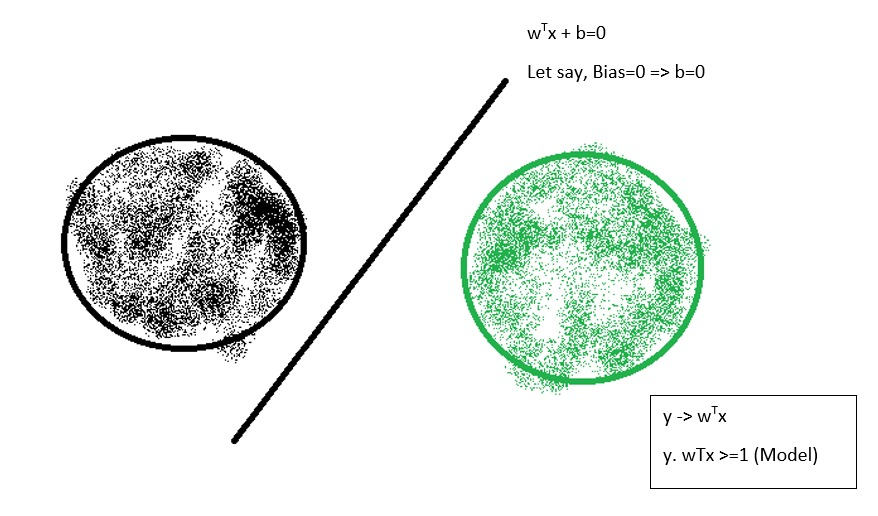
\includegraphics[scale=0.33]{419_1.jpeg}
\caption{}
\end{center}
\end{figure}

We are forcing the plane to pass through the origin, but these regions could be shifted.

\begin{figure}[htbp]
\begin{center}
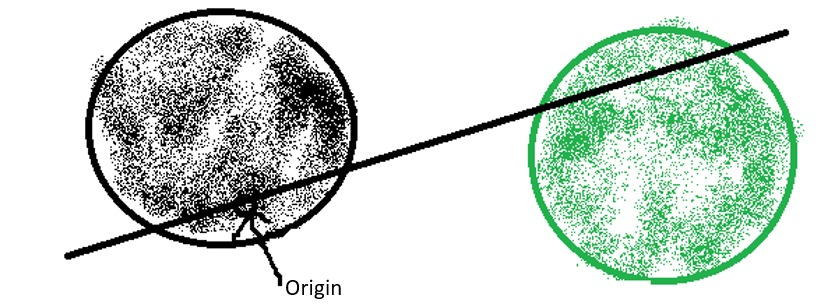
\includegraphics[scale=0.33]{419_2.jpeg}
\caption{}
\end{center}
\end{figure}

\subsubsection{Advantages of taking b=0}

Let us assume that bias is present
\begin{align}
{w^Tx} + b =0 \\
b \neq 0
\end{align}
\newpage
But now, we add a new point to Class 2 as shown below (figure 8.3).

\begin{figure}[htbp]
\begin{center}
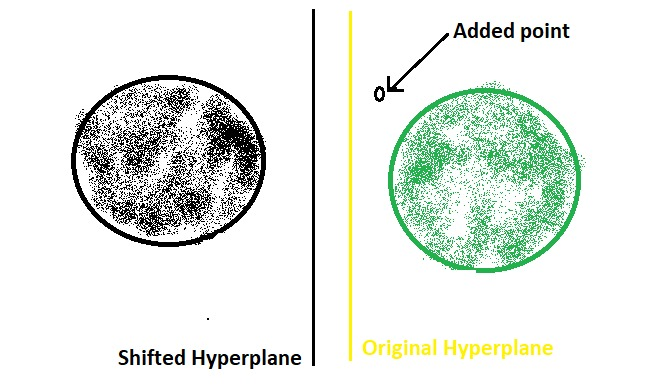
\includegraphics[scale=0.43]{419_3.jpeg}
\caption{}
\end{center}
\end{figure} 
It can be observed that even addition of a single point can lead to shifting of plane by a huge margin.\\ \\
\underline{Explanation}: The class 2 shifts more due to addition of the newly added point and thus ultimately the hyper-plane gets shifted more and the following problems can arise:
\begin{itemize}
    \item Not robust to outliers.
    \item Have generalisation issues like over-fitting.
    \item Model is super sensitive to addition of one point. Thus, privacy is at risk.
    Examples:
    \begin{itemize}
        \item When a patient data is added, model changes by a huge amount. We can reverse engineer the patient's data.
        \item Discussion of privacy issues with respect to data and tech companies like Google, Amazon and Facebook (Meta).
    \end{itemize}

\end{itemize}
Due to the above issues, the model is NOT stable.
\begin{figure}[htbp]
\begin{center}
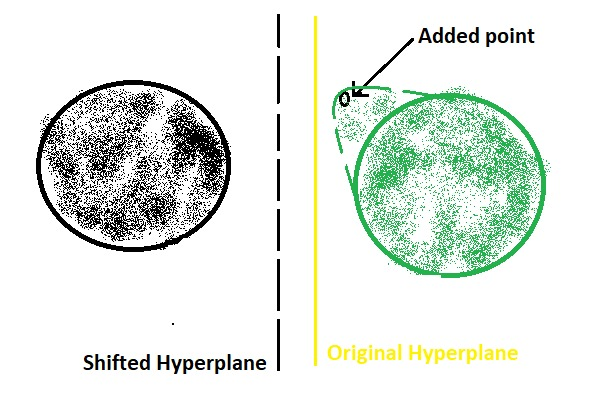
\includegraphics[scale=0.43]{419_4.jpeg}
\caption{}
\end{center}
\end{figure}


\subsection{Definition of Stability}

Let there be a dataset $D$, and algorithm $A$ and a singular point $a$. When a model is stable, the introduction of an additional point must result in a new model that only has a minute difference from the original model.
In particular for a  the following difference is small ($\O(\frac{1}{|D|})$):
$D \rightarrow A \rightarrow A(D)$ and $D\cup a \rightarrow A \rightarrow A(D\cup a)$. 

\subsection{Effect of Bias}
If we look at figure 8.2, we notice a considerable amount of incorrect classification. However, there is a bigger problem: the test set error is high. In figure 8.1, however, the test set error is low. Therefore the following inferences can be drawn for $y = sgn(w^Tx +b)$:
\begin{itemize}
    \item $b\neq 0$ improves the training accuracy but not necessarily the test accuracy. It is not stable (not robust to outliers and can result in privacy issues).
    \item $b=0$ does not improve training accuracy but may improve test accuracy. With the help of regularization, we can ensure stability and also generalise for real data (avoid over fitting).
\end{itemize}

\begin{figure}[htbp]
\begin{center}
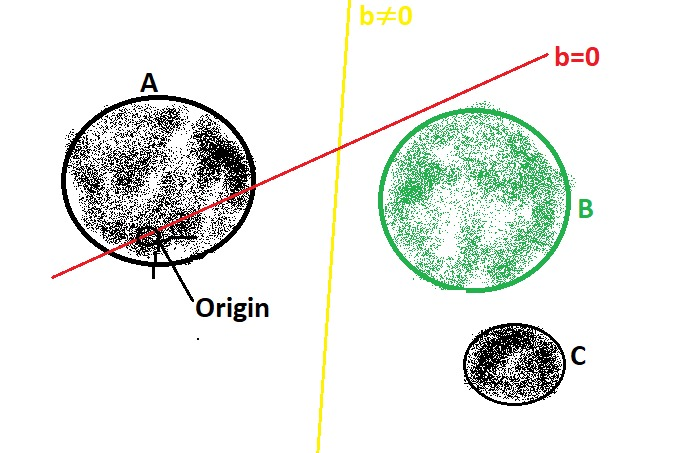
\includegraphics[scale=0.43]{419_5.jpeg}
\caption{}
\end{center}
\end{figure}
 
In figure 8.5, let the training set be A, B, C and the test set be A', B', C'. Then,\\ \begin{center}
    error(A', B', C' $ | b=0$) $\leq$ error(A', B', C' $| b\neq0$) - error(A, B, C $ | b\neq0$)
\end{center}
\subsection{Summary of the Above Discussion}
\begin{itemize}
    \item If the testing set (A', B', C') is similar to the test set (A, B, C), then $b\neq 0$ is better.
    \item If the test and training sets are different then $b=0$ will perform better as it will be more stable. However if this difference is large, then $b=0$ will NOT help.
\end{itemize}

\section{Summary}
In this note we look into the case of multi-class classification based on probabilistic models. We later discuss the concepts of stability and the effect of bias on the stability of the model in terms of shifting hyperplanes, training datasets and test datasets.

\section{Group Details}
\begin{itemize}
    \item 190100074	M Arvind
    \item 20D110002	Aarya Ajit Chaudhari
    \item 18D100007	Bhavini Jeloka
    \item 190100088	Parag Bajaj
    \item 200070061	Priyanshi Gupta
\end{itemize}

\end{document}





